\documentclass[10pt]{beamer}

% ==========================================
% Packages
% ==========================================
\usepackage{amsmath, amssymb}
\usepackage{tikz}
\usepackage{pgfplots}
\pgfplotsset{compat=1.17}
\usetikzlibrary{arrows.meta, positioning, shapes.geometric, decorations.pathreplacing, calc, shadows.blur}
\usepackage{listings}
\usepackage{xcolor}
\usepackage{booktabs}
\usepackage{adjustbox}

% Code listing style
\lstdefinestyle{cstyle}{
    backgroundcolor=\color{black!3},
    commentstyle=\color{green!50!black},
    keywordstyle=\color{blue!70!black}\bfseries,
    stringstyle=\color{red!70!black},
    basicstyle=\ttfamily\scriptsize,
    breakatwhitespace=false,
    breaklines=true,
    keepspaces=true,
    showspaces=false,
    showstringspaces=false,
    showtabs=false,
    tabsize=2,
    frame=single,
    framerule=0.2pt,
    rulecolor=\color{black!30},
    language=C
}
\lstset{style=cstyle}

% ==========================================
% Color definitions
% ==========================================
\definecolor{ntnured}{RGB}{180, 0, 0}
\definecolor{ntnugrey}{RGB}{210, 210, 210}
\definecolor{titlebg}{RGB}{248, 248, 248}
\definecolor{itemblue}{RGB}{60, 60, 140}
\definecolor{accentblue}{RGB}{30, 80, 160}
\definecolor{accentgreen}{RGB}{30, 130, 80}
\definecolor{accentorange}{RGB}{220, 130, 30}

% ==========================================
% Theme
% ==========================================
\usetheme{Boadilla}
\usecolortheme[named=ntnured]{structure}
% \useinnertheme[shadow]{rounded}

\setbeamercolor{title}{bg=titlebg, fg=ntnured}
\setbeamertemplate{title page}[default][rounded=true,shadow=true]

\setbeamertemplate{enumerate items}[ball]
\setbeamertemplate{itemize items}[ball]
\setbeamercolor{item projected}{bg=itemblue, fg=white}
\setbeamercolor{itemize item}{fg=itemblue}
\setbeamercolor{itemize subitem}{fg=itemblue!70}

% Custom blocks
\setbeamercolor{block title}{bg=ntnured!85, fg=white}
\setbeamercolor{block body}{bg=ntnured!5, fg=black}

% ==========================================
% Header
% ==========================================
\setbeamertemplate{headline}{
  \leavevmode%
  \hbox{%
  \begin{beamercolorbox}[wd=.5\paperwidth,ht=3ex,dp=1.25ex,left,leftskip=1em]{headline left}%
    \usebeamerfont{headline}\color{white}\textbf{\insertsectionhead}
  \end{beamercolorbox}%
  \begin{beamercolorbox}[wd=.5\paperwidth,ht=3ex,dp=1.25ex,right]{headline right}%
  \end{beamercolorbox}}%
  \vskip0pt%
}
\setbeamercolor{headline left}{bg=ntnured}
\setbeamercolor{headline right}{bg=ntnugrey}
\setbeamertemplate{navigation symbols}{}

% ==========================================
% Footer
% ==========================================
\setbeamertemplate{footline}{
  \leavevmode%
  \hbox{%
  \begin{beamercolorbox}[wd=.25\paperwidth,ht=2.25ex,dp=1ex,center]{author in head/foot}%
    \usebeamerfont{author in head/foot}\insertshortauthor
  \end{beamercolorbox}%
  \begin{beamercolorbox}[wd=.45\paperwidth,ht=2.25ex,dp=1ex,center]{title in head/foot}%
    \usebeamerfont{title in head/foot}\insertshorttitle
  \end{beamercolorbox}%
  \begin{beamercolorbox}[wd=.15\paperwidth,ht=2.25ex,dp=1ex,center]{date in head/foot}%
    \usebeamerfont{date in head/foot}\insertshortdate
  \end{beamercolorbox}%
  \begin{beamercolorbox}[wd=.15\paperwidth,ht=2.25ex,dp=1ex,right]{date in head/foot}%
    \insertframenumber{} / \inserttotalframenumber\hspace*{2ex}
  \end{beamercolorbox}}%
  \vskip0pt%
}

% ==========================================
% Title info
% ==========================================
\title[Cyber-Physical Systems]{CSC9008 Cyber-Physical Systems \\ Shake it off: Final Presentation}
\author[Hon, Wu, Lin]{
    \textmd{Course Instructor: Prof. Chao Wang} \\
    \vspace{0.4cm}
    \textmd{Students: Xin-Shao Hon, Zhen-Rong Wu, Darrin Lin}}
\institute[NTNU]{
  Department of Computer Science and Information Engineering \\
  National Taiwan Normal University \\
}
\date[June. 2, 2026]{June. 2, 2026}

\begin{document}

% =====================================================
% Title
% =====================================================
\begin{frame}
  \titlepage
\end{frame}

% =====================================================
% Outline
% =====================================================
\section{Outline}

\begin{frame}{Agenda}
  \begin{enumerate}
    \item System Architecture
    \item Recall: Basic background 
    \item Complementary Filter for Attitude Estimation
    \item PID Control System
    \item Cable-Length Geometry for MG90S Servos
    \item System analysis
    \item Live Demo
  \end{enumerate}
\end{frame}

% =====================================================
% 1. ARCHITECTURE
% =====================================================
\section{System Architecture}

\begin{frame}{Project Overview}
  \begin{block}{Goal}
    Build a self-stabilizing platform that keeps objects level despite external disturbances (manual tilting, vibration, earthquakes).
  \end{block}

  \begin{columns}[T,onlytextwidth]
    \column{0.48\textwidth}
    \textbf{Hardware:}
    \begin{itemize}
      \item STM32F401CCU6 (MCU)
      \item GY-521 / MPU6050 (IMU)
      \item 4 $\times$ MG90S servos
      \item Pulleys + strings
      \item Central universal joint
    \end{itemize}

    \column{0.48\textwidth}
    \textbf{Control flow:}
    \begin{itemize}
      \item Sense tilt via IMU
      \item Compute attitude (pitch, roll)
      \item PID computes correction
      \item Servos pull cables
      \item Platform tilts back to level
    \end{itemize}
  \end{columns}
\end{frame}

\begin{frame}{Hardware Price}
  \begin{center}
    \resizebox{0.9\textwidth}{!}{%
    \begin{tabular}{lccc}
      \toprule
      Component & Unit Price (NTD) & Quantity & Subtotal (NTD) \\
      \midrule
      STM32F401CCU6 & \$400 & 1 & \$400 \\
      GY-521 / MPU6050 & \$95 & 1 & \$95 \\
      MG90S Servo & \$50 & 4 & \$200 \\
      Clipboard & \$29 & 1 & \$29 \\
      Pulley  & \$19 & 4 & \$76 \\
      String & \$14 & 1 & \$14 \\
      Universal Joint  & \$76& 1 & \$76 \\
      Socket & \$23 & 1 & \$23 \\
      Screw Eye & \$12 & 1 pack & \$12 \\
      Serrated Flange Nut & \$20 & 1 pack & \$20 \\
      Washer & \$10 & 1 pack & \$10 \\
      Corrugated Board & \$12 & 1 & \$12 \\
      Acrylic Sheet & \$140 & 1 & \$140 \\
      Dupont Wires & \$20 & lots & \$20 \\
      Arduino Mega & \$400 & 1 & \$400 \\
      ST-link V2 & \$200 & 1 & \$200 \\
      \midrule
      \textbf{Total} & & & \textbf{\$1727} \\
      \bottomrule
\end{tabular}
    }
  \end{center}

\end{frame}

\begin{frame}{Quick Demo}
  \begin{center}

        \LARGE\textbf{Quick Live Demo} \\
        \normalsize (We will have a more detailed demo at the end of the presentation)

  \end{center}
\end{frame}

\begin{frame}{Mechanical Structure}
  \begin{center}
    \begin{tikzpicture}[scale=0.8, every node/.style={font=\footnotesize}]
      % Base
      \draw[fill=orange!20, draw=orange!80!black, thick]
        (-4, -2) rectangle (4, -1.7);
      \node[text=orange!60!black] at (0, -1.85) {\textbf{Base}};

      % Central pillar
      \draw[fill=gray!30, draw=black, thick, rotate=30] (-0.15, 0) rectangle (0.15, 0.5);
      \draw[fill=gray!30, draw=black, thick]
        (-0.15, -1.7) rectangle (0.15, 0);
      \node[anchor=west] at (0.2, -0.6)
      {Universal joint};

      % Joint sphere
      \draw[fill=gray!50, draw=black] (0, 0) circle (0.15);

      % Platform (tilted slightly)
      \draw[fill=blue!20, draw=blue!70!black, very thick, rotate around={10:(0, 0.5)}]
        (-3, 0.4) rectangle (3, 0.6);

      % Cup
      \draw[fill=brown!20, draw=brown!70!black, thick, rotate around={10:(0, 0.5)}]
        (-0.4, 0.6) rectangle (0.4, 1.2);
      \node[rotate=10] at (0, 0.9) {\tiny Cup};

      % Servos (left and right)
      \draw[fill=red!30, draw=red!70!black, thick]
        (-2, -1.7) rectangle (-2.5, -1.0);
      \draw[fill=red!30, draw=red!70!black, thick]
        (2.0, -1.7) rectangle (2.5, -1.0);
      \node[text=red!70!black] at (-2.25, -1.1) {\textbf{Servo}};
      \node[text=red!70!black] at (2.25, -1.1) {\textbf{Servo}};

      % Pulleys
      \draw[fill=yellow!50, draw=black] (-3, -1.5) circle (0.2);
      \draw[fill=yellow!50, draw=black] (3, -1.5) circle (0.2);

      % Cables (rotated platform endpoints)
      \draw[red!80!black, thick] (-3, 0.07) -- (-3, -1.5);
      \draw[red!80!black, thick] (3, 0.93) -- (3, -1.5);
      \draw[red!80!black, thick] (-3, -1.5) -- (-2.25, -1.5);
      \draw[red!80!black, thick] (3, -1.5) -- (2.25, -1.5);

      \draw[fill=green!30, draw=green!70!black, thick, rotate around={10:(0, 0.5)}]
        (-1.5, 0.2) rectangle (-0.9, 0.4);
      \node[rotate=10, text=green!50!black] at (-1.2, 0.1) {\tiny IMU};
｀
      % Annotations
      % \node[anchor=west, text=accentblue] at (3.5, 0.5) {$\theta$ tilt};
    \end{tikzpicture}
  \end{center}

  \begin{itemize}
    \item 4 cables pulling 4 platform corners (PA0 back, PA1 left, PA2 right, PA3 front)
    \item Cross-pairs work antagonistically: one pulls in, the other releases
    \item Central universal joint bears the load; servos only adjust angle
  \end{itemize}
\end{frame}

\begin{frame}{Signal Flow Diagram}
  \begin{center}
    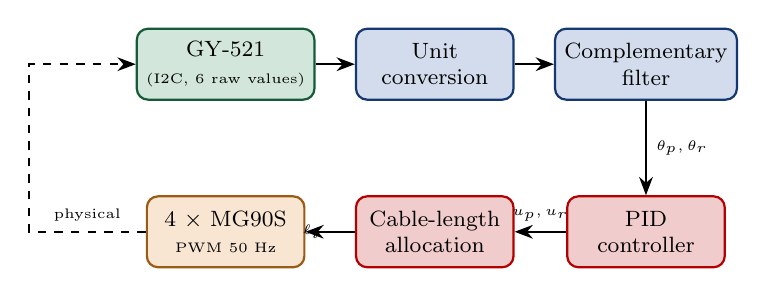
\begin{tikzpicture}[
      node distance=1.2cm and 0.5cm,
      block/.style={rectangle, draw, thick, rounded corners, minimum height=0.9cm, minimum width=2cm, font=\footnotesize, align=center},
      sensor/.style={block, fill=accentgreen!20, draw=accentgreen!70!black},
      proc/.style={block, fill=accentblue!20, draw=accentblue!70!black},
      ctrl/.style={block, fill=ntnured!20, draw=ntnured},
      act/.style={block, fill=accentorange!20, draw=accentorange!70!black},
      arr/.style={-Stealth, thick}
    ]
      \node[sensor] (imu) {GY-521 \\ \tiny (I2C, 6 raw values)};
      \node[proc, right=of imu] (conv) {Unit \\ conversion};
      \node[proc, right=of conv] (att) {Complementary \\ filter};
      \node[ctrl, below=of att] (pid) {PID \\ controller};
      \node[ctrl, below=of conv] (alloc) {Cable-length \\ allocation};
      \node[act, below=of imu] (servo) {4 $\times$ MG90S \\ \tiny PWM 50 Hz};

      \draw[arr] (imu) -- (conv);
      \draw[arr] (conv) -- (att);
      \draw[arr] (att) -- node[right, font=\tiny]{$\theta_p, \theta_r$} (pid);
      \draw[arr] (pid) -- node[above, font=\tiny]{$u_p, u_r$} (alloc);
      \draw[arr] (alloc) -- node[left, font=\tiny]{$\ell_i$} (servo);
      \draw[arr, dashed] (servo) -- node[above, font=\tiny]{physical} ++(-2.5, 0) |- (imu);
    \end{tikzpicture}
  \end{center}

  \begin{itemize}
    \item Closed-loop at \textbf{500 Hz} (2 ms control period)
    \item Pitch and roll axes controlled independently
    \item All computation runs on STM32F401, USB-CDC for logging
  \end{itemize}
\end{frame}



% =====================================================
% 5. MG90S geometry
% =====================================================
\section{Cable-Length Geometry for MG90S}

\begin{frame}{Geometric Setup of the Mechanism}
  \begin{center}
  \resizebox{0.95\textwidth}{!}{%
  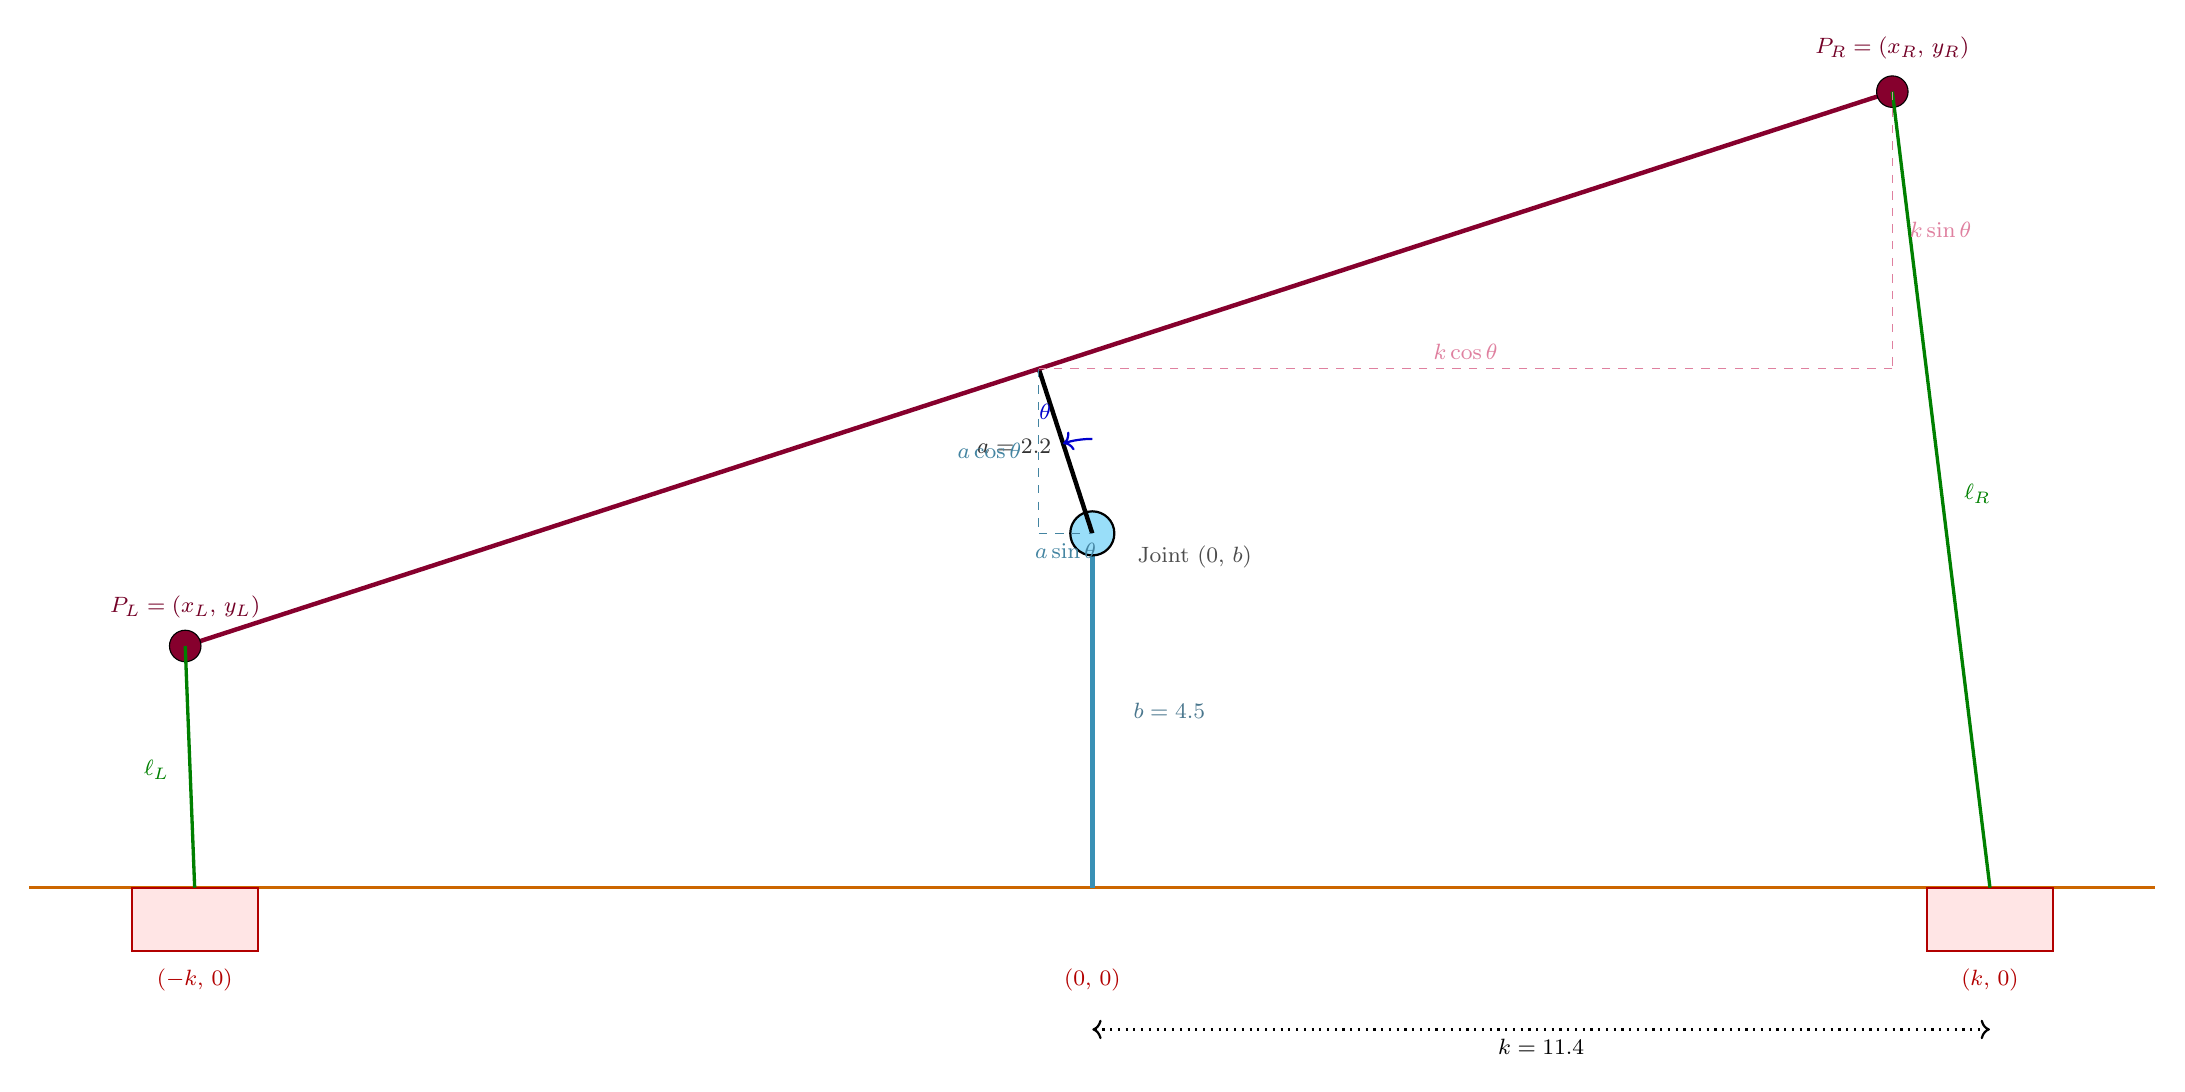
\begin{tikzpicture}[every node/.style={font=\footnotesize}]
    % Base
    \draw[orange!80!black, very thick] (-13.5, 0) -- (13.5, 0);

    % Servos
    \draw[fill=red!10, draw=red!70!black, thick]
      (-12.2, -0.8) rectangle (-10.6, 0);
    \draw[fill=red!10, draw=red!70!black, thick]
      (10.6, -0.8) rectangle (12.2, 0);
    \node[below=3pt, text=red!70!black] at (-11.4, -0.8) {$(-k,\,0)$};
    \node[below=3pt, text=red!70!black] at (11.4, -0.8) {$(k,\,0)$};
    \node[below=3pt, text=red!70!black] at (0, -0.8) {$(0,\,0)$};

    % Lower pillar (b)
    \draw[cyan!70!black, ultra thick] (0, 0) -- (0, 4.5);
    \node[text=cyan!50!black, anchor=west] at (0.4, 2.25) {$b = 4.5$};

    % Universal joint
    \draw[fill=cyan!40, draw=black, thick] (0, 4.5) circle (0.28);
    \node[anchor=west, text=black!70] at (0.45, 4.2) {Joint $(0,\,b)$};

    % Upper pillar (a), tilted by theta
    \draw[black, ultra thick] (0, 4.5) -- (-0.68, 6.59);
    \node[anchor=east, text=black!80] at (-0.4, 5.6) {$a = 2.2$};

    % Platform
    \draw[purple!70!black, ultra thick] (-11.52, 3.07) -- (10.16, 10.11);
    \draw[fill=purple!70!black] (-11.52, 3.07) circle (0.2);
    \draw[fill=purple!70!black] (10.16, 10.11) circle (0.2);
    \node[anchor=south, text=purple!60!black] at (10.16, 10.4)
      {$P_R = (x_R,\,y_R)$};
    \node[anchor=south, text=purple!60!black] at (-11.52, 3.3)
      {$P_L = (x_L,\,y_L)$};

    % Cables
    \draw[green!50!black, very thick] (-11.52, 3.07) -- (-11.4, 0);
    \draw[green!50!black, very thick] (10.16, 10.11) -- (11.4, 0);
    \node[text=green!50!black, anchor=east] at (-11.6, 1.5) {$\ell_L$};
    \node[text=green!50!black, anchor=west] at (10.95, 5) {$\ell_R$};

    % Theta arc
    \draw[->, thick, blue!80!black] (0, 5.7) arc (90:108:1.2);
    \node[text=blue!80!black] at (-0.6, 6.05) {$\theta$};

    % a*sin, a*cos
    \draw[dashed, cyan!60!black, thin] (-0.68, 6.59) -- (-0.68, 4.5);
    \draw[dashed, cyan!60!black, thin] (-0.68, 4.5) -- (0, 4.5);
    \node[text=cyan!60!black, anchor=east] at (-0.78, 5.55) {$a\cos\theta$};
    \node[text=cyan!60!black, anchor=north] at (-0.34, 4.5) {$a\sin\theta$};

    % k*sin, k*cos
    \draw[dashed, purple!50, thin] (10.16, 10.11) -- (10.16, 6.59);
    \draw[dashed, purple!50, thin] (10.16, 6.59) -- (-0.68, 6.59);
    \node[text=purple!50, anchor=south] at (4.74, 6.59) {$k\cos\theta$};
    \node[text=purple!50, anchor=west] at (10.26, 8.35) {$k\sin\theta$};

    % k width
    \draw[<->, dotted, thick] (0, -1.8) -- (11.4, -1.8);
    \node[anchor=north] at (5.7, -1.8) {$k = 11.4$};
  \end{tikzpicture}%
  }
  \end{center}
  \vspace{0.1cm}
  \scriptsize
  Platform tilts about the universal joint at $(0,b)$. The \emph{upper pillar} (length $a$) rigidly connects the joint to the platform center, so it tilts with the platform. Cables run from platform ends to fixed servos at $(\pm k, 0)$.
\end{frame}


\begin{frame}{Servo Action}
  Corrections $u_p$, $u_r$ in \textbf{degrees of attitude correction}.\\
  But each servo controls the \textbf{length of a cable} that pulls the platform.

  \begin{block}{Naive approach (does not work well)}
    Map servo angle directly to angle output: $\theta_{\text{servo}} += u$.\\
    Problem: $1^\circ$ of servo rotation does \emph{not} produce $1^\circ$ of platform tilt.
    The relationship is highly nonlinear because cables connect a rotating platform to fixed servo positions.
  \end{block}

  \begin{block}{Our approach}
    Compute the \emph{exact cable length} the platform would need at the desired tilt angle, then convert that length into a servo rotation via the spool radius.
  \end{block}
\end{frame}


\begin{frame}{Deriving the Cable Length (Step 1: Locate Platform Center)}
  The upper pillar rotates rigidly with the platform about the joint at $(0, b)$.

  The platform \emph{center} is the top of the upper pillar. Before rotation it sits at $(0, b+a)$. The offset from the joint is $(0, a)$. After rotation by $\theta$:
  \[
    \text{offset}' = \begin{bmatrix} \cos\theta & -\sin\theta \\ \sin\theta & \cos\theta \end{bmatrix} \begin{bmatrix} 0 \\ a \end{bmatrix}
    = \begin{bmatrix} -a\sin\theta \\ a\cos\theta \end{bmatrix}
  \]

  Add back the joint position $(0, b)$:
  \[
    \boxed{\;
      P_{\text{center}} = \bigl(-a\sin\theta,\; b + a\cos\theta\bigr)
    \;}
  \]

  \scriptsize
  This term is what makes our model different from a naive single-pillar setup. Because $a$ is not negligible compared to $k$, ignoring it would introduce a position error of up to $a\sin\theta_{\max}$ in the platform center.
\end{frame}

\begin{frame}{Deriving the Cable Length (Step 2: Platform Endpoints)}
  Each platform endpoint is offset $\pm k$ along the platform direction. After rotation, the offsets become $(\pm k\cos\theta,\; \pm k\sin\theta)$.

  Add to the platform center $P_{\text{center}}$:
  \[
    P_R = \bigl(-a\sin\theta + k\cos\theta,\; b + a\cos\theta + k\sin\theta\bigr)
  \]
  \[
    P_L = \bigl(-a\sin\theta - k\cos\theta,\; b + a\cos\theta - k\sin\theta\bigr)
  \]

  Cable length is the Euclidean distance from each endpoint to its servo:
  \[
    \ell_R = \|P_R - (k, 0)\|, \quad \ell_L = \|P_L - (-k, 0)\|
  \]

  \begin{block}{Result}
    \footnotesize
    \[
      \ell_R(\theta) = \sqrt{(-a\sin\theta + k\cos\theta - k)^2 + (b + a\cos\theta + k\sin\theta)^2}
    \]
    \[
      \ell_L(\theta) = \sqrt{(-a\sin\theta - k\cos\theta + k)^2 + (b + a\cos\theta - k\sin\theta)^2}
    \]
  \end{block}
\end{frame}

\begin{frame}{Sanity Check at $\theta = 0$}
  Substituting $\sin 0 = 0$, $\cos 0 = 1$:
  \[
    \ell_R(0) = \sqrt{(0 + k - k)^2 + (b + a + 0)^2} = a + b
  \]
  \[
    \ell_L(0) = \sqrt{(0 - k + k)^2 + (b + a - 0)^2} = a + b
  \]
  Both cables have length $a + b$ at rest \checkmark

  \medskip
  Cable length \emph{change} relative to neutral position:
  \[
    \Delta\ell_R(\theta) = \ell_R(\theta) - (a + b),
    \qquad
    \Delta\ell_L(\theta) = \ell_L(\theta) - (a + b)
  \]

  \begin{block}{Numerical example: $a=2.2$, $b=4.5$, $k=11.4$, $\theta=10^\circ$}
    \footnotesize
    \[
      \ell_R(10^\circ) \approx 8.66\ \text{cm},
      \quad \Delta\ell_R \approx +1.96\ \text{cm} \text{ (release)}
    \]
    \[
      \ell_L(10^\circ) \approx 4.69\ \text{cm},
      \quad \Delta\ell_L \approx -2.01\ \text{cm} \text{ (reel in)}
    \]
    The two cables move \emph{antagonistically} (one shortens, one lengthens) — exactly the behavior we want.
  \end{block}
\end{frame}

\begin{frame}{From Cable Length to Servo Angle}
  Each servo has a spool with circumference $C$. One full $360^\circ$ revolution winds/unwinds one full circumference of cable. Therefore:
  \[
    \Delta\ell = C \cdot \frac{\alpha}{360^\circ}
    \quad \Longrightarrow \quad
    \boxed{\;\alpha = \frac{360^\circ \cdot \Delta\ell}{C}\;}
  \]

  where $\alpha$ is the servo rotation (in degrees) and $\Delta\ell$ is the required cable-length change.

  \medskip
  Final servo command (relative to the $90^\circ$ neutral position):
  \[
    \theta_{\text{servo}} = 90^\circ + \alpha
  \]

  \begin{block}{Continuing the example ($\Delta\ell_R = +1.96$ cm, $C = 2\pi r$ with $r = 1.0$ cm $\Rightarrow C \approx 6.28$ cm)}
    \footnotesize
    \[
      \alpha_R = \frac{360 \cdot 1.96}{6.28} \approx 112^\circ
    \]
    A 112$^\circ$ servo rotation is required to release 1.96 cm of cable — which is why bigger spool circumference gives finer (but smaller-range) control.
  \end{block}
\end{frame}


% =====================================================
% 2. MPU6050
% =====================================================
\section{MPU6050: Reading and Parsing Sensor Data}

\begin{frame}{What the MPU6050 Measures}
  \begin{block}{Two sensors in one chip}
    \textbf{Accelerometer:} measures \emph{specific force} (in g)\\
    \textbf{Gyroscope:} measures \emph{angular rate} (in deg/s)
  \end{block}

  \begin{columns}[T,onlytextwidth]
    \column{0.5\textwidth}
    \textbf{Accelerometer (counter-intuitive!)}\\
    Even when stationary, the chip reads $1\,g$ on $z$ because:
    \[
      \vec{a}_{\text{meas}} = \vec{a}_{\text{motion}} - \vec{g}
    \]
    The spring inside resists gravity $\Rightarrow$ measurement is the reaction force.

    \column{0.5\textwidth}
    \begin{center}
    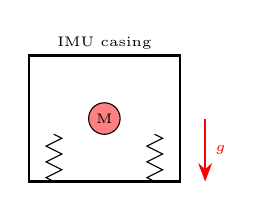
\begin{tikzpicture}[scale=0.8]
      \draw[thick] (-1.2, -1) rectangle (1.2, 1);
      \node at (0, 1.2) {\tiny IMU casing};
      \draw[fill=red!50] (0, 0) circle (0.25);
      \node at (0, 0) {\tiny M};
      \foreach \x in {-0.8, 0.8} {
        \draw[decorate, decoration={zigzag, segment length=2mm, amplitude=1mm}]
          (\x, -1) -- (\x, -0.25);
      }
      \draw[-Stealth, thick, red] (1.6, 0) -- (1.6, -1) node[midway, right] {\tiny $g$};
    \end{tikzpicture}
    \end{center}
  \end{columns}
\end{frame}

% \begin{frame}[fragile]{I2C Communication and Raw Data Format}
%   Each axis returns a \textbf{16-bit signed integer} (range $-32768 \sim +32767$).
%   Six axes packed in 14 bytes starting at register \texttt{0x3B}:

%   \begin{center}
%   \scriptsize
%   \begin{tabular}{cccccccc}
%     \toprule
%     Reg & 0x3B--3C & 0x3D--3E & 0x3F--40 & 0x41--42 & 0x43--44 & 0x45--46 & 0x47--48 \\
%     Data & ACCEL\_X & ACCEL\_Y & ACCEL\_Z & TEMP & GYRO\_X & GYRO\_Y & GYRO\_Z \\
%     \bottomrule
%   \end{tabular}
%   \end{center}

% \begin{lstlisting}
% uint8_t buf[14];
% HAL_I2C_Mem_Read(&hi2c1, 0xD0, 0x3B, 1, buf, 14, 100);
% int16_t ax_raw = (int16_t)((buf[0] << 8) | buf[1]);
% int16_t ay_raw = (int16_t)((buf[2] << 8) | buf[3]);
% int16_t az_raw = (int16_t)((buf[4] << 8) | buf[5]);
% int16_t gx_raw = (int16_t)((buf[8] << 8) | buf[9]);
% int16_t gy_raw = (int16_t)((buf[10] << 8) | buf[11]);
% int16_t gz_raw = (int16_t)((buf[12] << 8) | buf[13]);
% \end{lstlisting}
% \end{frame}

% \begin{frame}{Converting Raw Counts to Physical Units}
%   \begin{block}{Accelerometer ($\pm 2\,g$ range)}
%     Full scale: $-32768 \leftrightarrow -2g$, $+32767 \leftrightarrow +2g$
%     \[
%       1 \text{ raw unit} = \frac{2g - (-2g)}{65536} = \frac{1g}{16384}
%     \]
%     \[
%       \boxed{a_{[g]} = \frac{a_{\text{raw}}}{16384}}
%     \]
%   \end{block}

%   \begin{block}{Gyroscope ($\pm 250$ deg/s range)}
%     \[
%       1 \text{ raw unit} = \frac{500\, \text{deg/s}}{65536} \approx \frac{1\, \text{deg/s}}{131}
%     \]
%     \[
%       \boxed{\omega_{[\text{deg/s}]} = \frac{\omega_{\text{raw}}}{131}}
%     \]
%   \end{block}

%   \scriptsize
%   \textbf{Sanity check (flat, stationary):} $a_x \approx 0$, $a_y \approx 0$, $a_z \approx 1\,g$ (raw $\approx 16384$).
% \end{frame}

% \begin{frame}[fragile]{Initialization and Calibration}
%   \textbf{Step 1: Wake up the chip (it boots in sleep mode!)}

% \begin{lstlisting}
% uint8_t d = 0x01;  // X-gyro clock source, wake up
% HAL_I2C_Mem_Write(&hi2c1, 0xD0, 0x6B, 1, &d, 1, 100);
% // SMPLRT_DIV = 7  -> sample rate 125 Hz
% // CONFIG     = 3  -> DLPF cutoff ~44 Hz (Fourier!)
% // GYRO_CFG   = 0  -> +/- 250 deg/s
% // ACCEL_CFG  = 0  -> +/- 2g
% \end{lstlisting}

%   \textbf{Step 2: Static calibration}\\
%   Average $N = 1000$ samples at rest to estimate the constant bias:
%   \[
%     a_{\text{off}} = \frac{1}{N}\sum_{k=1}^{N} a_k - \begin{bmatrix} 0\\0\\1 \end{bmatrix},
%     \qquad
%     \omega_{\text{off}} = \frac{1}{N}\sum_{k=1}^{N} \omega_k
%   \]

%   Every subsequent reading subtracts this offset:
%   \[
%     a_{\text{corrected}} = \frac{a_{\text{raw}}}{16384} - a_{\text{off}}
%   \]
% \end{frame}

% =====================================================
% 3. COMPLEMENTARY FILTER
% =====================================================
\section{Complementary Filter}

\begin{frame}{Fuse Two Sensors}
  \begin{center}
  \footnotesize
  \begin{tabular}{lcc}
    \toprule
     & \textbf{Accelerometer} & \textbf{Gyroscope} \\
    \midrule
    Steady state & Accurate (gravity) & Slow drift \\
    Fast motion & Corrupted by inertia & Accurate \\
    Long term & No drift & Drift grows with $t$ \\
    \midrule
    Good in & Low frequency & High frequency \\
    \bottomrule
  \end{tabular}
  \end{center}

  \begin{block}{Key Idea}
    Use accelerometer for low-frequency reference (gravity is reliable)\\
    Use gyroscope for high-frequency dynamics (no motion artefacts)\\
    Blend them with a \textbf{frequency-domain crossover} $\Rightarrow$ Complementary Filter
  \end{block}

  \scriptsize
  Kalman filter would adapt the weights dynamically, but the fixed-weight complementary filter is sufficient for our low-speed platform and is far cheaper computationally (1 multiply + 1 add per axis).
\end{frame}

% \begin{frame}{Attitude from Accelerometer Alone}
%   \textbf{Setup:} Gravity in the world frame, $z$-axis up:
%   \[
%     \vec{g}_W = \begin{bmatrix} 0\\0\\-g \end{bmatrix}
%   \]
%   When the platform rotates by pitch $\theta_p$ (around $y$) and roll $\theta_r$ (around $x$), the IMU sees gravity rotated into its body frame.

%   \begin{block}{Rotation matrix (passive, body-frame view)}
%     \[
%       R(\theta_p, \theta_r) = R_x(\theta_r)\, R_y(\theta_p)
%     \]
%     \[
%       \vec{g}_{\text{IMU}} = R \cdot \vec{g}_W
%     \]
%   \end{block}

%   Since $\vec{g}_W$ has only a $z$-component, only the third column of $R$ survives.\\
%   After multiplication:
%   \[
%     \begin{aligned}
%       a_x &= \sin\theta_p \\
%       a_y &= -\sin\theta_r \cos\theta_p \\
%       a_z &= \cos\theta_r \cos\theta_p
%     \end{aligned}
%     \qquad (\text{in units of } g)
%   \]
% \end{frame}

% \begin{frame}{Deriving the Pitch/Roll Formulas}
%   Combine $a_y^2 + a_z^2$ to isolate $\theta_p$:
%   \[
%     a_y^2 + a_z^2 = \sin^2\theta_r\cos^2\theta_p + \cos^2\theta_r\cos^2\theta_p = \cos^2\theta_p
%   \]

%   Therefore $\sqrt{a_y^2+a_z^2} = \cos\theta_p$, and
%   \[
%     \tan\theta_p = \frac{a_x}{\sqrt{a_y^2+a_z^2}}
%   \]

%   \begin{block}{Final attitude equations (use \texttt{atan2} for full-quadrant range)}
%     \[
%       \theta_p^{\text{acc}} = \mathrm{atan2}\!\left(a_x,\; \sqrt{a_y^2 + a_z^2}\right)
%     \]
%     \[
%       \theta_r^{\text{acc}} = \mathrm{atan2}\!\left(-a_y,\; a_z\right)
%     \]
%   \end{block}

%   \scriptsize
%   \textbf{Verification (flat):} $a_x{=}0, a_y{=}0, a_z{=}1 \Rightarrow \theta_p = \theta_r = 0$. \checkmark\\
%   \textbf{Verification (pitch 30$^\circ$):} $a_x{=}0.5, a_z{=}0.866 \Rightarrow \theta_p = \mathrm{atan2}(0.5, 0.866) = 30^\circ$. \checkmark
% \end{frame}

% \begin{frame}{The Gyroscope Path}
%   The gyroscope reports angular rate $\omega$. To get an angle, integrate:
%   \[
%     \theta^{\text{gyro}}(t) = \theta(0) + \int_0^t \omega(\tau)\,d\tau
%   \]
%   Discrete form (sample every $\Delta t = 5$ ms):
%   \[
%     \theta_k^{\text{gyro}} = \theta_{k-1} + \omega_k \cdot \Delta t
%   \]

%   \begin{block}{Drift problem}
%     Any constant bias $b$ in $\omega_{\text{meas}} = \omega_{\text{true}} + b$ grows linearly:
%     \[
%       \theta_k^{\text{gyro}} = \theta_{\text{true}}(t) + b\cdot t
%     \]
%     A 0.05 deg/s bias becomes $3^\circ$ after one minute.
%   \end{block}

%   $\Rightarrow$ Gyroscope alone diverges. Accelerometer alone is too noisy.\\
%   $\Rightarrow$ We need to fuse them.
% \end{frame}

% \begin{frame}{The Complementary Filter}
%   \begin{block}{Discrete recursion}
%     \[
%       \boxed{\;
%       \hat{\theta}_k = \alpha\!\left(\hat{\theta}_{k-1} + \omega_k \Delta t\right) + (1 - \alpha)\,\theta_k^{\text{acc}}
%       \;}
%     \]
%   \end{block}

%   \begin{itemize}
%     \item $\alpha \approx 0.98$: trust gyroscope short-term, use accelerometer to slowly correct drift.
%     \item Equivalent to: \textbf{high-pass on gyro + low-pass on accel}, summing to unity gain.
%   \end{itemize}

%   \textbf{Crossover frequency (Fourier interpretation):}
%   \[
%     f_c = \frac{1 - \alpha}{2\pi\,\alpha\,\Delta t}
%     = \frac{0.02}{2\pi \cdot 0.98 \cdot 0.005}
%     \approx 0.65\ \text{Hz}
%   \]

%   \scriptsize
%   Below 0.65 Hz: accel dominates (gravity reference); above: gyro dominates (fast motion).
% \end{frame}

% \begin{frame}{Filter Behavior (Conceptual)}
%   \begin{center}
%   \begin{tikzpicture}
%     \begin{axis}[
%       width=10cm, height=5cm,
%       xlabel={Frequency (Hz, log scale)},
%       ylabel={Gain},
%       xmode=log, xmin=0.01, xmax=100,
%       ymin=0, ymax=1.2,
%       grid=both,
%       legend pos=south east,
%       legend style={font=\tiny}
%     ]
%       \addplot[blue, very thick, domain=0.01:100, samples=200] {1/sqrt(1 + (x/0.65)^2)};
%       \addplot[red, very thick, domain=0.01:100, samples=200] {(x/0.65)/sqrt(1 + (x/0.65)^2)};
%       \addplot[black, dashed] coordinates {(0.65, 0) (0.65, 1.2)};
%       \node[anchor=south] at (axis cs:0.65, 1.05) {\scriptsize $f_c = 0.65$ Hz};
%       \legend{Low-pass (Accel weight), High-pass (Gyro weight)}
%     \end{axis}
%   \end{tikzpicture}
%   \end{center}

%   \begin{itemize}
%     \item Sum of both curves equals 1 at every frequency $\Rightarrow$ \emph{complementary}
%     \item No phase distortion at the crossover
%     \item One tuning parameter ($\alpha$), trivial to implement
%   \end{itemize}
% \end{frame}

% \begin{frame}[fragile]{Implementation}
% \begin{lstlisting}
% #define ALPHA  0.98f
% #define DT     0.005f   // 200 Hz control loop
% #define R2D    (180.0f / 3.14159265f)

% void Attitude_Update(Attitude_t *a, MPU6050_t *imu) {
%     // Accel-based static angle
%     float pitch_acc = atan2f(-imu->ax,
%         sqrtf(imu->ay*imu->ay + imu->az*imu->az)) * R2D;
%     float roll_acc  = atan2f(imu->ay, imu->az) * R2D;

%     // Complementary filter
%     a->pitch = ALPHA * (a->pitch + imu->gx * DT)
%              + (1.0f - ALPHA) * pitch_acc;
%     a->roll  = ALPHA * (a->roll  + imu->gy * DT)
%              + (1.0f - ALPHA) * roll_acc;
% }
% \end{lstlisting}

%   \scriptsize
%   Gyro-to-axis mapping (gx vs gy, and sign) is determined experimentally because it depends on how the IMU is physically oriented on the platform.
% \end{frame}

% =====================================================
% 4. PID
% =====================================================
\section{PID Control System}

\begin{frame}{Control Problem Statement}
  \begin{block}{Objective}
    Drive the platform attitude $(\theta_p, \theta_r)$ to $(0, 0)$ in the presence of disturbances.
  \end{block}

  Define the error signal:
  \[
    e(t) = \theta_{\text{ref}}(t) - \theta(t) = 0 - \theta(t) = -\theta(t)
  \]

  We want a control law $u(t)$ (servo correction in degrees) that:
  \begin{itemize}
    \item Reacts quickly to disturbances
    \item Eliminates steady-state error (when the table itself is tilted)
    \item Avoids overshoot and oscillation
  \end{itemize}

  $\Rightarrow$ \textbf{PID controller}, the workhorse of feedback control (Week 11).
\end{frame}

\begin{frame}{The Three Terms of PID}
  \begin{block}{Continuous form}
    \[
      u(t) = \underbrace{K_p\, e(t)}_{\text{Proportional}}
           + \underbrace{K_i \int_0^t e(\tau)\,d\tau}_{\text{Integral}}
           + \underbrace{K_d\, \frac{de(t)}{dt}}_{\text{Derivative}}
    \]
  \end{block}

  \footnotesize
  \begin{tabular}{c|p{3.2cm}|p{3.2cm}|p{2.5cm}}
    \toprule
    Term & Reacts to & Cures & Side effect \\
    \midrule
    P & Current error & Slow response & Steady-state error \\
    I & Accumulated error & Steady-state error & Overshoot, slow \\
    D & Rate of change of error & Overshoot, damping & Noise amplification \\
    \bottomrule
  \end{tabular}

  \vspace{0.4cm}
  Analogy:\\
  P = spring (pulls toward target),\quad
  D = damper (resists motion),\quad
  I = memory (accumulates over time)
\end{frame}

\begin{frame}{Why I Eliminates Steady-State Error}
  Apply the \textbf{Final Value Theorem}:
  \[
    e_{ss} = \lim_{t\to\infty} e(t) = \lim_{s\to 0} s\, E(s)
  \]

  For a step disturbance $T_d(s) = T_0/s$ with PI(D) control:
  \[
    e_{ss} = \lim_{s\to 0} \frac{s \cdot T_0/s}{1 + G_p(s)C(s)}
          = \frac{T_0}{1 + \lim_{s\to 0} G_p(s)C(s)}
  \]

  Since $C(s)$ contains $K_i/s$, $\lim_{s\to 0} C(s) = \infty$, therefore:
  \[
    \boxed{\; e_{ss} = 0 \;}
  \]

  \scriptsize
  Without the I term, $\lim_{s\to 0} C(s) = K_p$ is finite, yielding a non-zero steady-state error.
  This is the mathematical reason we need the integral term.
\end{frame}

\begin{frame}{Discrete Implementation}
  Approximate the integral by rectangular sum, derivative by backward difference:
  \[
    \int_0^{t_k} e\,d\tau \approx \sum_{i=0}^{k} e_i \Delta t,
    \qquad
    \frac{de}{dt} \approx \frac{e_k - e_{k-1}}{\Delta t}
  \]

  \begin{block}{Discrete PID}
    \[
      u_k = K_p\, e_k + K_i \cdot \Delta t \sum_{i=0}^{k} e_i + K_d \cdot \frac{e_k - e_{k-1}}{\Delta t}
    \]
  \end{block}

  \textbf{Two practical safeguards:}
  \begin{itemize}
    \item \textbf{Anti-windup:} clip the integral so it cannot grow unboundedly during saturation
    \item \textbf{Output saturation:} clip $u$ to the servo's physical range
  \end{itemize}
\end{frame}



\begin{frame}{Discrete Velocity Form: PI Implementation}
  \textbf{Standard Velocity Form PID:}
  Subtracting positional $u_{k-1}$ from $u_k$ yields the required \textit{change} $\Delta u_k$:
  \[
    \Delta u_k = u_k - u_{k-1} = K_p[e_k - e_{k-1}] + K_i e_k + K_d[e_k - 2e_{k-1} + e_{k-2}]
  \]

  \vspace{0.3cm}
  
  \begin{block}{Our Velocity Form PI Implementation}
    To avoid noise amplification from the second difference (D term), our firmware omits the $K_d$ term and implements a \textbf{Velocity Form PI} controller:
    \[
      \Delta u_k = K_{P\_vel}\,[e_k - e_{k-1}] + K_{I\_vel}\, e_k
    \]
  \end{block}
  
  \vspace{0.2cm}
  \footnotesize
  \textbf{Engineering Insight:} In microcontrollers, the second difference $[e_k - 2e_{k-1} + e_{k-2}]$ is highly sensitive to sensor noise. Dropping it ensures a smoother control signal.
\end{frame}


\begin{frame}{Velocity Form PI: Mathematical Equivalence}
  \textbf{Why does it work? (When Accumulated)}
  
  Accumulating (integrating) the velocity step $\Delta u_k$ over time mathematically reconstructs the standard positional control law:
  \[
    u_k = \sum_{j=0}^{k} \Delta u_j = K_{P\_vel}\, e_k + K_{I\_vel} \sum_{j=0}^{k} e_j
  \]

  \vspace{0.2cm}
  
  \begin{itemize}

    \item \textbf{$K_{P\_vel}$ acts as Proportional ($P$):} \\
    Multiplies the first difference $[e_k - e_{k-1}]$. When accumulated, the intermediate terms cancel out (telescoping sum), leaving just the current error $e_k$.
    
    \vspace{0.2cm}
    
    \item \textbf{$K_{I\_vel}$ acts as Integral ($I$):} \\
    Multiplies the current error $e_k$ directly. When summed over time, it naturally becomes the accumulated historical error ($\sum e_j$).
  \end{itemize}
\end{frame}


% \begin{frame}[fragile]{Implementation in C}
% \begin{lstlisting}
% float PID_compute(float setpoint, float measured,
%                   float *integral, float *prev_err,
%                   float Kp, float Ki, float Kd, float dt)
% {
%     float err = setpoint - measured;

%     // Integral term with anti-windup
%     *integral += err * dt;
%     if (*integral >  I_LIMIT) *integral =  I_LIMIT;
%     if (*integral < -I_LIMIT) *integral = -I_LIMIT;

%     // Derivative term
%     float deriv = (err - *prev_err) / dt;
%     *prev_err = err;

%     // PID output with saturation
%     float u = Kp*err + Ki*(*integral) + Kd*deriv;
%     if (u >  OUT_LIMIT) u =  OUT_LIMIT;
%     if (u < -OUT_LIMIT) u = -OUT_LIMIT;
%     return u;
% }
% \end{lstlisting}

%   \scriptsize
%   Two independent PIDs run in parallel: one for pitch, one for roll.
% \end{frame}


\begin{frame}{Full Control Pipeline}
  \begin{enumerate}
    \item Read IMU, compute $\theta_p$ and $\theta_r$ via complementary filter.
    \item Run two independent PIDs:
      \[ u_p = \mathrm{PID}_p(0 - \theta_p), \quad u_r = \mathrm{PID}_r(0 - \theta_r) \]
    \item For each axis, compute the required cable lengths using the geometric formulas:
      \[ \ell_R = \ell_R(u_p), \quad \ell_L = \ell_L(u_p) \]
    \item Convert each cable length to a servo rotation:
      \[ \alpha_i = \frac{360^\circ \cdot \bigl(\ell_i - (a+b)\bigr)}{C} \]
    \item Output PWM via TIM2 channels.
  \end{enumerate}

  Same procedure runs for the roll axis.\\
  All computations complete within one 5 ms control period.
\end{frame}

\end{document}